\chapter{Adaptive Beamforming Background}
\label{chap:abf_background}

\section{Introduction}

In this section, the concept of beamforming, and its method of adaptation, is introduced. It's assumed the reader is familiar with fundamental discrete signal processing techniques, such as Finite Impulse Response (FIR) filtering.

\section{Beamforming}

In signal processing, filtering is a fairly common operation; in the discrete sense, samples are passed through a set of filter coefficients, or "taps", to perform the convolution and acheive the desired response. Analagous to such temporal filtering, an array of sensors can be filtered \emph{spatially} to produce a desired response across the elements.

Specifically in the context of Radio Frequency (RF) antenna arrays, this spatial filtering can be utilized to optimize the overall antenna pattern, in a process commonly known as \emph{beamforming}\citep{van_veen_and_buckley}. The specific spatial optimization is often application dependent, however beamforming is generally seen as a method of beam steering, where gain is provided in a specific, desired direction, with attenuation in other locations. Though the term "beamforming" sounds like a specific application of array radiation, beamforming- and spatial filtering- can be performed on both the transmit and receive functions of an array.

blah double cite \citep{Alexander_and_Ghirnikar,Haykin}

As seen in Figure \ref{fig:ula_beamformer}

\begin{figure}[!htbp]
  \centering
  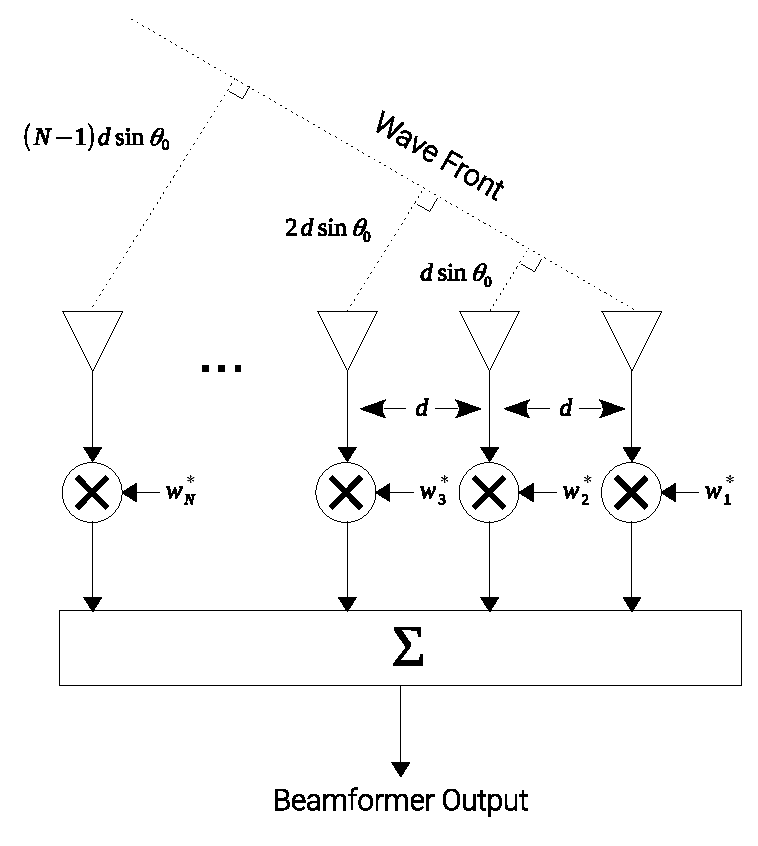
\includegraphics[]{02_abf_background/ula_beamformer}
  \caption{ULA Beamformer}
  \label{fig:ula_beamformer}
\end{figure}

\subsection{Adaptive Beamforming}

A standard beamformer, with pre-determined beamforming weights, can be called a \emph{deterministic beamformer} \citep{6206403}. For MIMO communication arrays, the properties of direction gain and attenuation can be exploited for servicing multiple users, such as in Spatial Multiplexing \citep{6732923}.

Though

\subsection{QR Decomposition}

hello \citep{AN506}


